\documentclass[12pt,a4paper]{article}

\usepackage[utf8]{inputenc}
\usepackage[margin=1in]{geometry}
\usepackage{amsmath,amssymb,amsfonts}
\usepackage{graphicx}
\usepackage{booktabs}
\usepackage{tikz}
\usetikzlibrary{shapes.geometric, arrows.meta, positioning, shadows, fit, backgrounds}
\usepackage{hyperref}
\usepackage{listings}
\usepackage{xcolor}
\usepackage{fancyhdr}

\hypersetup{
    colorlinks=true,
    linkcolor=blue!70!black,
    citecolor=blue!70!black,
    urlcolor=blue!70!black
}

\definecolor{codegreen}{rgb}{0,0.6,0}
\definecolor{codegray}{rgb}{0.5,0.5,0.5}
\definecolor{codepurple}{rgb}{0.58,0,0.82}
\definecolor{backcolour}{rgb}{0.96,0.96,0.96}

\lstdefinestyle{mystyle}{
    backgroundcolor=\color{backcolour},   
    commentstyle=\color{codegreen},
    keywordstyle=\color{blue},
    numberstyle=\tiny\color{codegray},
    stringstyle=\color{codepurple},
    basicstyle=\ttfamily\footnotesize,
    breakatwhitespace=false,         
    breaklines=true,                 
    captionpos=b,                    
    keepspaces=true,                 
    numbers=left,                    
    numbersep=5pt,                  
    showspaces=false,                
    showstringspaces=false,
    showtabs=false,                  
    tabsize=2
}
\lstset{style=mystyle}

\pagestyle{fancy}
\fancyhf{}
\rhead{GAI-PLA Project Documentation}
\lhead{Generative AI Personalized Learning Agent}
\cfoot{\thepage}

\begin{document}

% -----------------------------------------------------------------------------
% Title Page
% -----------------------------------------------------------------------------
\begin{titlepage}
    \centering
    \vspace*{1.5cm}
    
    {\Huge \textbf{GAI-PLA}}\\[0.4cm]
    {\LARGE \textbf{Generative AI-Based Personalized Learning Agent}}\\[1.2cm]
    
    \textbf{Final Year Capstone Project Technical Documentation}\\[2.5cm]
    
    \begin{minipage}{0.48\textwidth}
        \begin{flushleft} \large
            \textbf{Student Name:}\\
            Anurag Gaur\\
            \vspace{0.3cm}
            \textbf{Repository:}\\
            \href{https://github.com/anuraggaur29/GAI-PLA}{\texttt{github.com/anuraggaur29/GAI-PLA}}
        \end{flushleft}
    \end{minipage}
    \hfill
    \begin{minipage}{0.48\textwidth}
        \begin{flushright} \large
            \textbf{Academic Year:}\\
            2025--2026\\[0.3cm]
            \textbf{Domain:}\\
            Artificial Intelligence in Education (AI-Ed) / LLM Systems
        \end{flushright}
    \end{minipage}
    
    \vfill
    {\large Department of Computer Science \& Engineering}\\[0.2cm]
    {\large University Final Year Project Report}
\end{titlepage}

\tableofcontents
\newpage

% -----------------------------------------------------------------------------
% Abstract
% -----------------------------------------------------------------------------
\begin{abstract}
Personalized education demands scalable architectures that dynamically calibrate instructional difficulty, track student mastery across sessions, and produce structured, multi-format pedagogical content on demand. This report presents \textbf{GAI-PLA} (\textit{Generative AI-Based Personalized Learning Agent}), an end-to-end intelligent tutoring system built on a directed acyclic LangGraph state machine, powered by Google Gemini via an OpenAI-compatible structured gateway, and integrated with a decoupled vector memory store. Starting solely from an arbitrary subject query (e.g., \textit{``Pythagoras theorem''}), GAI-PLA constructs a hierarchical Knowledge Graph, executes an adaptive diagnostic quiz, evaluates concept-level deficiencies, and generates customized remedial Markdown lessons and 16:9 presentation slide decks with native PPTX export. The system features pluggable pedagogy styles (Feynman, Socratic, and Scaffolding) and an Ebbinghaus-decayed L2 reflection memory loop.
\end{abstract}

% -----------------------------------------------------------------------------
% Chapter 1: Introduction
% -----------------------------------------------------------------------------
\section{Introduction}

\subsection{Motivation and Problem Statement}
Traditional computer-aided instruction (CAI) platforms suffer from two major limitations:
\begin{enumerate}
    \item \textbf{Static Content Bottlenecks:} Conventional systems rely on pre-curated question banks and static textbook chapters, limiting their ability to synthesize ad-hoc curriculum on emerging or interdisciplinary topics.
    \item \textbf{Memory-Deficient Tutoring:} Standard Large Language Model (LLM) chat interfaces operate in conversational silos without persistent mastery modeling, leading to redundant explanations or miscalibrated difficulty.
\end{enumerate}

\subsection{Project Objectives}
The core objectives of the \textbf{GAI-PLA} architecture are:
\begin{itemize}
    \item \textbf{Zero-Cold-Start Curriculum Generation:} Convert any input query into an organized, multi-node Knowledge Graph (KG) with prerequisites and sub-skills.
    \item \textbf{Calibrated Formative Assessment:} Dynamically generate diagnostic items targeted to specific graph nodes to pinpoint exact learner misconceptions.
    \item \textbf{Multi-Format Remediation:} Concurrently synthesize interactive text lessons and structured slide presentations ($1000 \times 562.5$ canvas layout) exported directly to PowerPoint (\texttt{.pptx}).
    \item \textbf{Swappable Pedagogy:} Decouple instructional strategies from code, enabling real-time switching between Feynman Technique, Socratic Dialogue, and Cognitive Scaffolding.
\end{itemize}

% -----------------------------------------------------------------------------
% Chapter 2: System Architecture
% -----------------------------------------------------------------------------
\section{System Architecture}

GAI-PLA is structured as a decoupled full-stack architecture comprising a high-throughput FastAPI backend, a LangGraph state machine, an OpenAI-compatible LLM orchestration layer, and an optional HNSW vector memory microservice.

\begin{figure}[htbp]
\centering
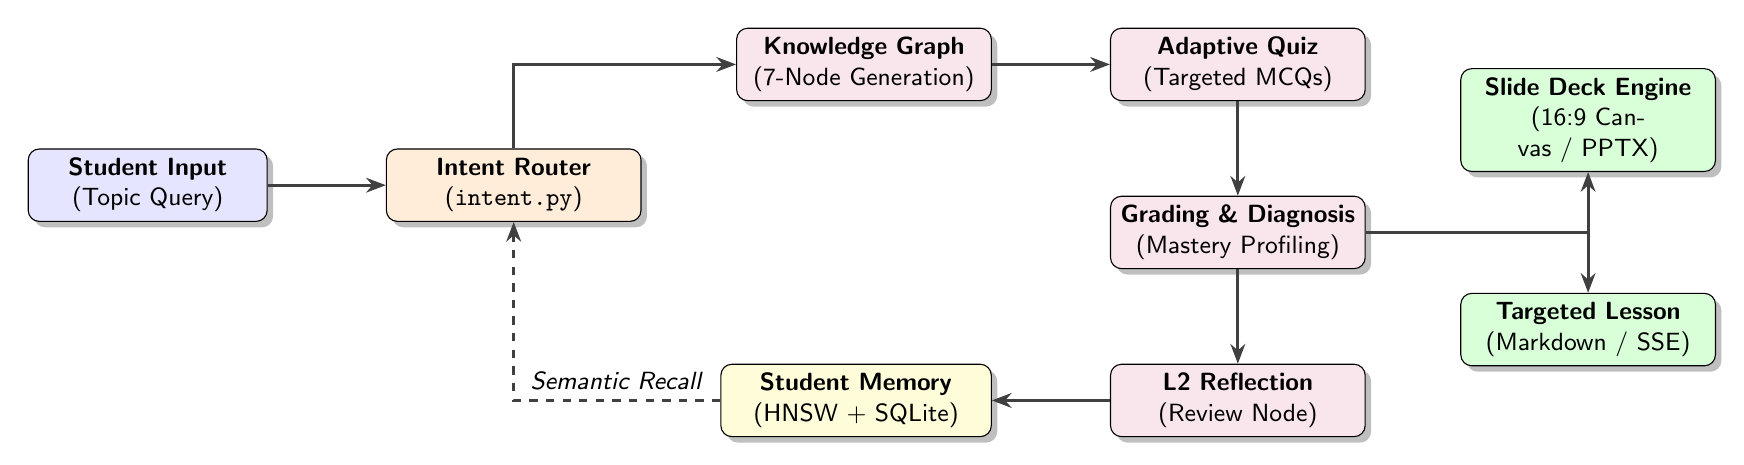
\begin{tikzpicture}[
    node distance=1.2cm and 1.5cm,
    font=\small\sffamily,
    base/.style={draw, rounded corners=4pt, align=center, fill=white, drop shadow},
    userNode/.style={base, fill=blue!10, text width=2.8cm, minimum height=0.9cm},
    routerNode/.style={base, fill=orange!15, text width=3.0cm, minimum height=0.9cm},
    procNode/.style={base, fill=purple!10, text width=3.0cm, minimum height=0.9cm},
    outputNode/.style={base, fill=green!15, text width=3.0cm, minimum height=0.9cm},
    memNode/.style={base, fill=yellow!15, text width=3.2cm, minimum height=0.9cm},
    arrow/.style={-{Stealth[length=2.5mm]}, line width=1.1pt, draw=black!75}
]

% Nodes
\node (user) [userNode] {\textbf{Student Input}\\(Topic Query)};
\node (intent) [routerNode, right=of user] {\textbf{Intent Router}\\(\texttt{intent.py})};

\node (kg) [procNode, above right=0.6cm and 1.2cm of intent] {\textbf{Knowledge Graph}\\(7-Node Generation)};
\node (quiz) [procNode, right=of kg] {\textbf{Adaptive Quiz}\\(Targeted MCQs)};
\node (diag) [procNode, below=of quiz] {\textbf{Grading \& Diagnosis}\\(Mastery Profiling)};

\node (lesson) [outputNode, below right=0.3cm and 1.2cm of diag] {\textbf{Targeted Lesson}\\(Markdown / SSE)};
\node (slides) [outputNode, above right=0.3cm and 1.2cm of diag] {\textbf{Slide Deck Engine}\\(16:9 Canvas / PPTX)};

\node (review) [procNode, below=1.2cm of diag] {\textbf{L2 Reflection}\\(Review Node)};
\node (memory) [memNode, left=of review] {\textbf{Student Memory}\\(HNSW + SQLite)};

% Paths
\draw [arrow] (user) -- (intent);
\draw [arrow] (intent) |- (kg);
\draw [arrow] (kg) -- (quiz);
\draw [arrow] (quiz) -- (diag);
\draw [arrow] (diag) -| (lesson);
\draw [arrow] (diag) -| (slides);
\draw [arrow] (diag) -- (review);
\draw [arrow] (review) -- (memory);
\draw [arrow, dashed] (memory) -| node[pos=0.25, above] {\textit{Semantic Recall}} (intent);

\end{tikzpicture}
\caption{End-to-End Execution Flow of the GAI-PLA Learning Loop.}
\label{fig:arch_flow}
\end{figure}

\subsection{LangGraph Execution Engine}
The backend orchestrates instructional stages using a unified execution state defined by \texttt{LearningState} (Pydantic schema). HTTP requests trigger single-round state transitions:
\begin{equation}
\mathcal{S}_{t+1} = \mathcal{T}(\mathcal{S}_t, \mathcal{I}_t)
\end{equation}
where $\mathcal{S}_t$ represents the current pedagogical state (active graph, question queue, student responses, diagnosed weak points) and $\mathcal{I}_t$ is the user intent resolved by the LLM.

\subsection{Pluggable Pedagogy Layer}
Pedagogical methodologies are isolated in filesystem-level descriptors (\texttt{skills/<pedagogy>/SKILL.md}), eliminating the need to alter application logic when injecting novel instructional paradigms:
\begin{itemize}
    \item \textbf{Feynman Technique:} Forces simple language, intuitive analogies, and plain-term summaries of complex principles.
    \item \textbf{Socratic Method:} Withholds direct solutions; prompts the learner with targeted counter-questions to induce self-guided discovery.
    \item \textbf{Scaffolding:} Breaks complex problem-solving sequences into tiered cognitive steps, withdrawing assistance as mastery increases.
\end{itemize}

% -----------------------------------------------------------------------------
% Chapter 3: Implementation Details
% -----------------------------------------------------------------------------
\section{Implementation Details}

\subsection{LLM Gateway \& Structured Validation}
GAI-PLA interacts with Google Gemini models via an OpenAI-compatible REST endpoint (\texttt{https://generativelanguage.googleapis.com/v1beta/openai/}). To guarantee deterministic execution across JSON-parsing boundaries, the client wraps raw HTTP completions with the \textbf{Instructor} library:

\begin{lstlisting}[language=Python, caption={LLM Client Configuration with Structured Pydantic Output}]
def get_llm_client() -> instructor.Instructor:
    base_client = openai.OpenAI(
        api_key=os.environ.get("OPENAI_API_KEY"),
        base_url=os.environ.get("OPENAI_BASE_URL"),
        http_client=httpx.Client(trust_env=False, timeout=120.0)
    )
    return instructor.from_openai(base_client)
\end{lstlisting}

Every generated artifact—including multiple-choice items (\texttt{QuizQuestion}), node relations (\texttt{KnowledgeGraph}), and presentation elements (\texttt{SlideData})—undergoes rigid Pydantic model validation prior to UI delivery.

\subsection{Slide Post-Processing Chain}
Synthesizing slide presentations directly from generative models frequently introduces boundary overflows and LaTeX syntax errors. GAI-PLA enforces a deterministic 5-stage layout post-processing chain:
\begin{equation}
\text{Raw JSON} \xrightarrow{\text{Repair}} \text{Defaults} \xrightarrow{\text{LaTeX Parser}} \text{Bounds Enforcement } (1000 \times 562.5) \xrightarrow{\text{ID Assignment}} \text{Valid Canvas}
\end{equation}

% -----------------------------------------------------------------------------
% Chapter 4: Case Study & Empirical Results
% -----------------------------------------------------------------------------
\section{Experimental Case Study: Pythagoras Theorem}

To evaluate system efficacy, an end-to-end learning trial was executed on the topic \textit{``Pythagoras theorem''}.

\subsection{Phase 1: Knowledge Graph Synthesis}
The system decomposed the subject into 7 interconnected concept nodes:
\begin{itemize}
    \item \textit{Right Triangle}, \textit{Area of a Square}, \textit{Squares and Square Roots}, \textit{Pythagorean Theorem}, \textit{Pythagorean Triples}, \textit{Distance Formula}, and \textit{Basics of Trigonometry}.
\end{itemize}

\subsection{Phase 2: Formative Assessment \& Diagnosis}
An adaptive 14-question diagnostic quiz was evaluated:
\begin{table}[htbp]
\centering
\caption{Diagnostic Assessment Results by Knowledge Component}
\label{tab:eval_results}
\begin{tabular}{lccc}
\toprule
\textbf{Knowledge Component} & \textbf{Items Tested} & \textbf{Correct} & \textbf{Mastery Status} \\
\midrule
Pythagorean Theorem & 2 & 2 & Mastered (100\%) \\
Right Triangle & 2 & 0 & Deficient (Needs Review) \\
Area of a Square & 2 & 1 & Partial (Needs Review) \\
Squares and Square Roots & 2 & 1 & Partial (Needs Review) \\
Pythagorean Triples & 2 & 1 & Partial (Needs Review) \\
Distance Formula & 2 & 1 & Partial (Needs Review) \\
Basics of Trigonometry & 2 & 1 & Partial (Needs Review) \\
\midrule
\textbf{Overall Diagnostic Score} & \textbf{14} & \textbf{7} & \textbf{50\% Accuracy} \\
\bottomrule
\end{tabular}
\end{table}

\subsection{Phase 3: Targeted Remediation}
Upon identifying specific deficiencies (notably 0/2 on \textit{Right Triangle}), GAI-PLA bypassed mastered concepts and automatically formulated targeted remedial content focusing on fundamental hypotenuse relationships, producing:
\begin{enumerate}
    \item A formatted Markdown lesson delivered via live Server-Sent Events (SSE).
    \item A 16:9 presentation slide deck exported to \texttt{.pptx}.
\end{enumerate}

% -----------------------------------------------------------------------------
% Chapter 5: Conclusion & Future Scope
% -----------------------------------------------------------------------------
\section{Conclusion and Future Scope}

GAI-PLA establishes a resilient, production-ready framework for adaptive generative education. By combining LangGraph state determinism, Instructor schema validation, and real-time frontend streaming, the platform eliminates hallucination cascades and delivers structured learning paths from bare topic queries.

Future extensions include:
\begin{itemize}
    \item Full local activation of multi-lingual embedding pipelines (\texttt{bge-m3}) within \texttt{student\_memory}.
    \item Automated generation of interactive 3D visualizations for STEM topics via Three.js.
    \item Multimodal voice synthesis for conversational tutoring interactions.
\end{itemize}

% -----------------------------------------------------------------------------
% References
% -----------------------------------------------------------------------------
\begin{thebibliography}{99}
\bibitem{langgraph} LangChain Team, \emph{LangGraph: Multi-Agent Orchestration Framework}, 2024.
\bibitem{gemini} Google DeepMind, \emph{Gemini Models: Technological Report}, 2024.
\bibitem{instructor} J. Zhang, \emph{Instructor: Structured Data Extraction for LLMs}, 2024.
\bibitem{ebbinghaus} H. Ebbinghaus, \emph{Memory: A Contribution to Experimental Psychology}, Teachers College, Columbia University, 1913.
\end{thebibliography}

\end{document}
